\section{Introduction}
\label{sec:intro}

% Key/value stores remain a fundamental building block of modern
% scale-out service architectures.  Recent trends in primary storage
% technologies, however, are pushing operators to consider ever-more
% disaggregated designs for their in-memory storage systems.
% Concretely, increases in CPU core counts coupled with stagnating DRAM
% density has led to an increased interest in remote memory tiers, where
% some portion of memory is connected to the server over a network.
% Moreover, once disaggregated, memory can be pooled to achieve greater
% cost and power efficiencies.  The challenge facing fully disaggregated
% memory pools, however, is managing concurrent updates in the face of
% client failures and high access latencies.

% While cache-coherent technologies like CXL are beginning to
% become available, RDMA remains the commodity option for
% large-scale in-memory key/value stores.
% Many prior RDMA-based systems opt for a partially
% disaggregated model, in which a CPU core is collocated with
% remote memory to provide the needed
% serialization~\cite{erpc,herd,pilaf,cell,clover,sherman}.
% Fully disaggregated systems rely upon one-sided RDMA atomic
% operations (e.g., compare-and-swap) to resolve data
% races~\cite{rolex,fusee,race} which constrains their design.
% Specifically, RDMA atomic operations can act upon 64 contiguous bits
% of memory at a time at most, leading to implementations that employ
% multi-stage datastructures to support practical key and value sizes.

% In general, existing systems rely upon a high-performance index
% structure to localize key operations and maintain values separately,
% necessitating multiple RDMA operations and network round trips even in
% the absence of contention.  Moreover, given the dominance of
% read-heavy workloads~\cite{rocks-db-workload,facebook-memcached}, most
% systems eschew locks in favor of optimistic update approaches that can
% lead to poor performance under contention.
% In this work we design an index datastructure tailored for the
% constraints of current RDMA hardware.  Specifically, we
% facilitate lock-based updates by decreasing the number of round
% trips required to acquire locks and perform mutating operations.

Disaggregated architectures aim to improve resource scalability and utilization by pooling network
attached resources~\cite{dredbox,firebox,blade-server,legoos}. Pools reduce resource fragmentation,
stranding, and enable datacenter operators to provision for the sum-of-peak workloads rather than
the peak-of-sums~\cite{dsnf,supernic}. DRAM pooling is particularly attractive due to diminishing
improvements in its density but simultaneously difficult as local DRAM access latencies are much
lower than even the fastest RDMA
networks~\cite{fastswap,3po,kona,infiniswap,hydra,leap,legoos,dilos}.

Sharing disaggregated memory is fundamentally hard because cost of synchronization is high.  Most
systems choose to statically partition memory and optimize by reducing remote accesses through a
variety of techniques (cache policy, compilers, pointer
analysis~\cite{kona,mira,aifm,trackfm,carbink}). In contrast, disaggregated key-value stores (KVS)
both pool and share memory with a consistent read and write
interface~\cite{rolex,smart,ditto,fusee,clover,sherman,ford}.

The core challenging in designing a disaggregated KVS is efficient serialization. Memory
disaggregation assumes that machines housing pooled DRAM do not have CPUs powerful enough to service
requests. Thus, clients must implement their own serialization protocols. These protocols use
one-sided RDMA and carefully coordinate reads, writes, and atomic operations to maximize operations
per second.  The choice between lock-based and lock-free synchronization is an extremely delicate
one. But one which typically falls on semantic lines. KVS's with ordered keys (BTrees \& Radix
Trees) use locks~\cite{sherman,smart}, while those with unordered keys choose lock-free
techniques~\cite{rolex,ditto,fusee,clover}. In general the cost of lock-based approaches is
considered too high for unordered KVS due to critical section size, RDMA atomic bottlenecks, and
complex failure scenarios. Indeed, all lock based KVS's to date assume that clients are co-located
to combine writes, and do not provide a fault-tolerance protocol~\cite{sherman,smart}.

In this work we take the view that lock-based synchronization can provide very high performance for
unordered KVS's. We argue that because locks enable inlined operations on KVS indexes which can
result in significantly faster reads on common mixed read and write workloads by reducing round
trips. Further, locks enable the use of established RDMA KVS algorithms like Cuckoo hashing. We show
that atomic operation bottlenecks can be entirely avoided by using a NIC-based lock table, and that
through fine grained locking and careful protocol design critical sections can be reduced to a
single round trip in the common case and achieve high performance without co-locating clients.
Finally we demonstrate that a leased based lock acquisition protocol can be used to provide
fault-tolerance in the face of client failures with held locks.  To demonstrate the effectiveness of
our approach we introduce RCuckoo, a fully disaggregated KVS based on cuckoo hashing~\cite{cuckoo}.
RCuckoo builds around a novel \emph{dependent hashing} algorithm that makes spatial locality a
tunable parameter. Locality is the linchpin of our design as it enables us to efficiently determine
the ranges of memory each operation needs and acquire the right locks.



\begin{figure*}[t]
    \centering
    \newcommand{\subfigwidth}{0.32\linewidth}
    % \begin{subfigure}{\subfigwidth}
    %     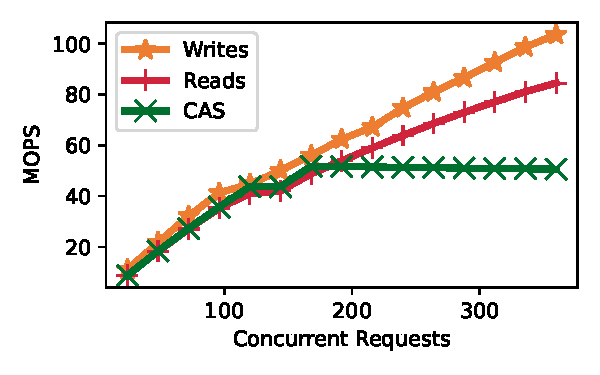
\includegraphics[width=0.99\linewidth]{fig/rdma_concur.pdf}
    %     % \label{fig:optimistic_failures}
    %     % \caption{}
    % \end{subfigure}
    \begin{subfigure}{\subfigwidth}
        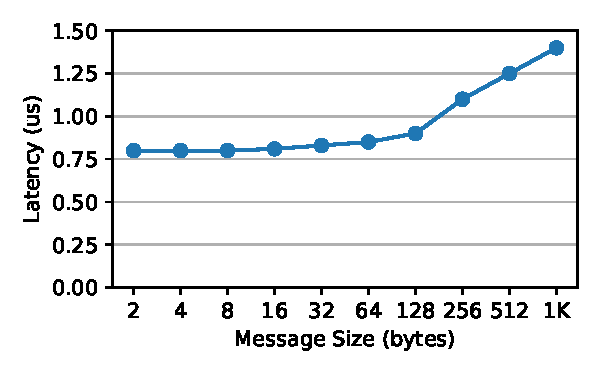
\includegraphics[width=0.99\linewidth]{fig/rdma_latency.pdf}
    \end{subfigure}
    \begin{subfigure}{\subfigwidth}
      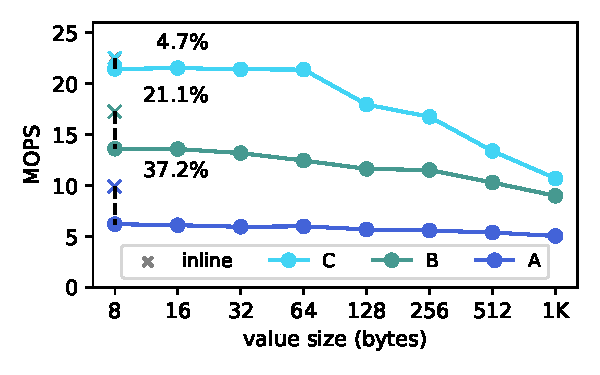
\includegraphics[width=0.99\linewidth]{fig/extent.pdf}
    \end{subfigure}
    \begin{subfigure}{\subfigwidth}
        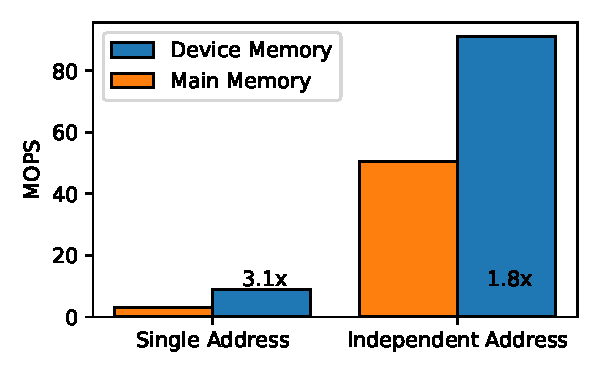
\includegraphics[width=0.99\linewidth]{fig/rdma_cas_throughput.pdf}
    \end{subfigure}
    \vspace{-1em}
    \caption{Basic RDMA performance on our testbed.
    % \textbf{(a)} (64-bit) operations per second;
    \textbf{(a)} operation latency as a function of message size~\cite{rdma-latency}; and
    \textbf{(b)} Extent vs Inline performance on YCSB workloads for small values (C=100\% reads, B=95\%read 5\%write A=50\%read 50\% write).
    \textbf{(c)} compare-and-swap performance on device and main memory.
    }
    \label{fig:rdma-benchmarks}
\vskip -1em
\end{figure*}

Combined with a datastructure design that facilitates aggressive batching of RDMA operations, these
techniques enable RCuckoo to limit the number of round trips required for all table operations.  In
the common case, reads execute in one or two (for large values) round trips, uncontested updates and
deletes require two round trips, and the median insert operation involves only two round
trips---although the expected number increases as the table fills.  On our testbed, RCuckoo delivers
comparable or higher performance on small values across the standard set  of YCSB benchmarks than
all of the existing disaggregated key/value stores we consider.  Concretely, with 320 clients
RCuckoo delivers up to a 2.5$\times$ throughput improvement on read-intensive (YCSB-B) workloads and
up to 7.1$\times$ their throughput on write-intensive (YCSB-A) workloads.  Moreover, RCuckoo's
performance remains high despite 100s of clients failing per second.
